\section{Homografija i transformacija perspektive}

Rezultat procesa uparivanja značajki je skup parova odgovarajućih točaka između referentne slike i slike dobivene sa kamere, no taj skup gotovo uvijek sadrži i određeni broj pogrešnih podudaranja. Te pogreške nastanu zbog dvosmislenosti ili nesavršenosti SIFT deskriptora. Kako bi se uspostavila pouzdana geometrijska veza između dviju slika potrebno je pronaći matematički model koji opisuje transformaciju tih slika, ali na način koji je robustan na prisutnost tih pogrešnih parova. Takav model je homografija. 

Homografija je projektivna transformacija u 2D prostoru koja preslikava točke iz jedne ravnine u drugu. U ovom slučaju te ravnine su referentna slika i slika dobivena sa kamere. Homografija se može opisati 3x3 matričnom jednadžbom
\begin{equation}
    s *
    \begin{pmatrix}
        x' \\
        y' \\
        1
    \end{pmatrix}
    =
    \begin{pmatrix}
        h_1 & h_2 & h_3 \\
        h_4 & h_5 & h_6 \\
        h_7 & h_8 & h_9
    \end{pmatrix}
    \begin{pmatrix}
        x \\
        y \\
        1
    \end{pmatrix}
\end{equation}
gdje su $x$ i $y$ koordinate točke na referentnoj slici, a $x'$ i $y'$ koordinate točke na slici dobivenoj sa kamere. $s$ predstavlja faktor skale tj. $s$ je posljedica korištenja homogenih koordinata i predstavlja treću komponentu rezultirajućeg vektora prije normalizacije. Faktor $s$ osigurava da jednadžba vrijedi u projektivnom prostoru. Matrica $H$ je homografska matrica koja se sastoji od 9 koeficijenata, no $h_9$ je tipično postavljen na 1 što znači da matrica ima 8 stupnjeva slobode. Za njen izračun potrebno je poznavati barem 4 odgovarajuće točke na referentnoj i slici dobivenoj sa kamere, pod uvjetom da su točke nekolinearne.
Budući da za izračun homografije potrebno je samo četri para točaka, a iz procesa uparivanja dobije se znatno više parova, potrebno je odabrati najbolje parove na način da se također eliminira utjecaj pogrešnih podudaranosti. Za rješavanje ovog problema koristi se RANSAC (eng. \textit{Random Sample Consensus}) algoritam. RANSAC je iterativni algoritam koji se sastoji od sljedećih koraka. 
Prvo se nasumično odabire minimalni podskup podataka potreban za izračun homografije, odnosno četri para uparenih točaka. Na temelju tih nasumičnih točaka izračunava se preliminarna homografija $H$. Potom se ta preliminarna homografija testira na način da se ta matrica primjenjuje na sve ostale točke iz početnog seta podataka i određuje se udaljenost između izračunate točke i prave točke iz seta. Ako je ta udaljenost manja od predefiniranog praga onda se taj par smatra podudaranim s modelom. Cijeli ovaj postupak se ponavlja veliki broj puta. 
Na kraju se odabire matrica H koja je u jednoj od iteracija dobila najveći broj podudaranja s modelom. Korištenjem ovog algoritma osigurava se da pogrešne podudaranosti budu efikasno ignorirane jer se neće uklopiti u jedan konzistentan geometrijski model.

Primjer matrice homografije dobivene iz procesa uparivanja značajki prikazanog na slici~\ref{fig:uparivanje_znacajki} može izgledati ovako:

\begin{equation}
    H =
    \begin{pmatrix}
        0.6298 & 0.0750 & 412.29 \\
        0.0065 & 0.7816 & 271.09 \\
        0.000000280 & 0.0000741 & 1
    \end{pmatrix}
\end{equation}

Ova matrica $H$ transformira koordinate točaka s referentne slike penjačkog smjera na sliku dobivenu sa kamere, uzimajući u obzir rotaciju, translaciju, skaliranje i perspektivnu deformaciju. Vrijednosti u matrici su stvarni primjer dobiven iz procesa uparivanja značajki za konkretni slučaj prikazan u prethodnom poglavlju.




Kada je pronađena matrica $H$ s njom se može postići transformacija perspektive između dviju slika. Korištenjem homografije moguće je preslikati referentnu sliku linije penjačkog smjera na sliku dobivenu sa kamere koristeći OpenCV biblioteku te algoritam \textit{warpPerspective}. Kao izlaz, generira se nova slika na kojoj je sadržaj perspektivno izobličen u skladu s matricom $H$. 

\begin{figure}[H]
    \centering
    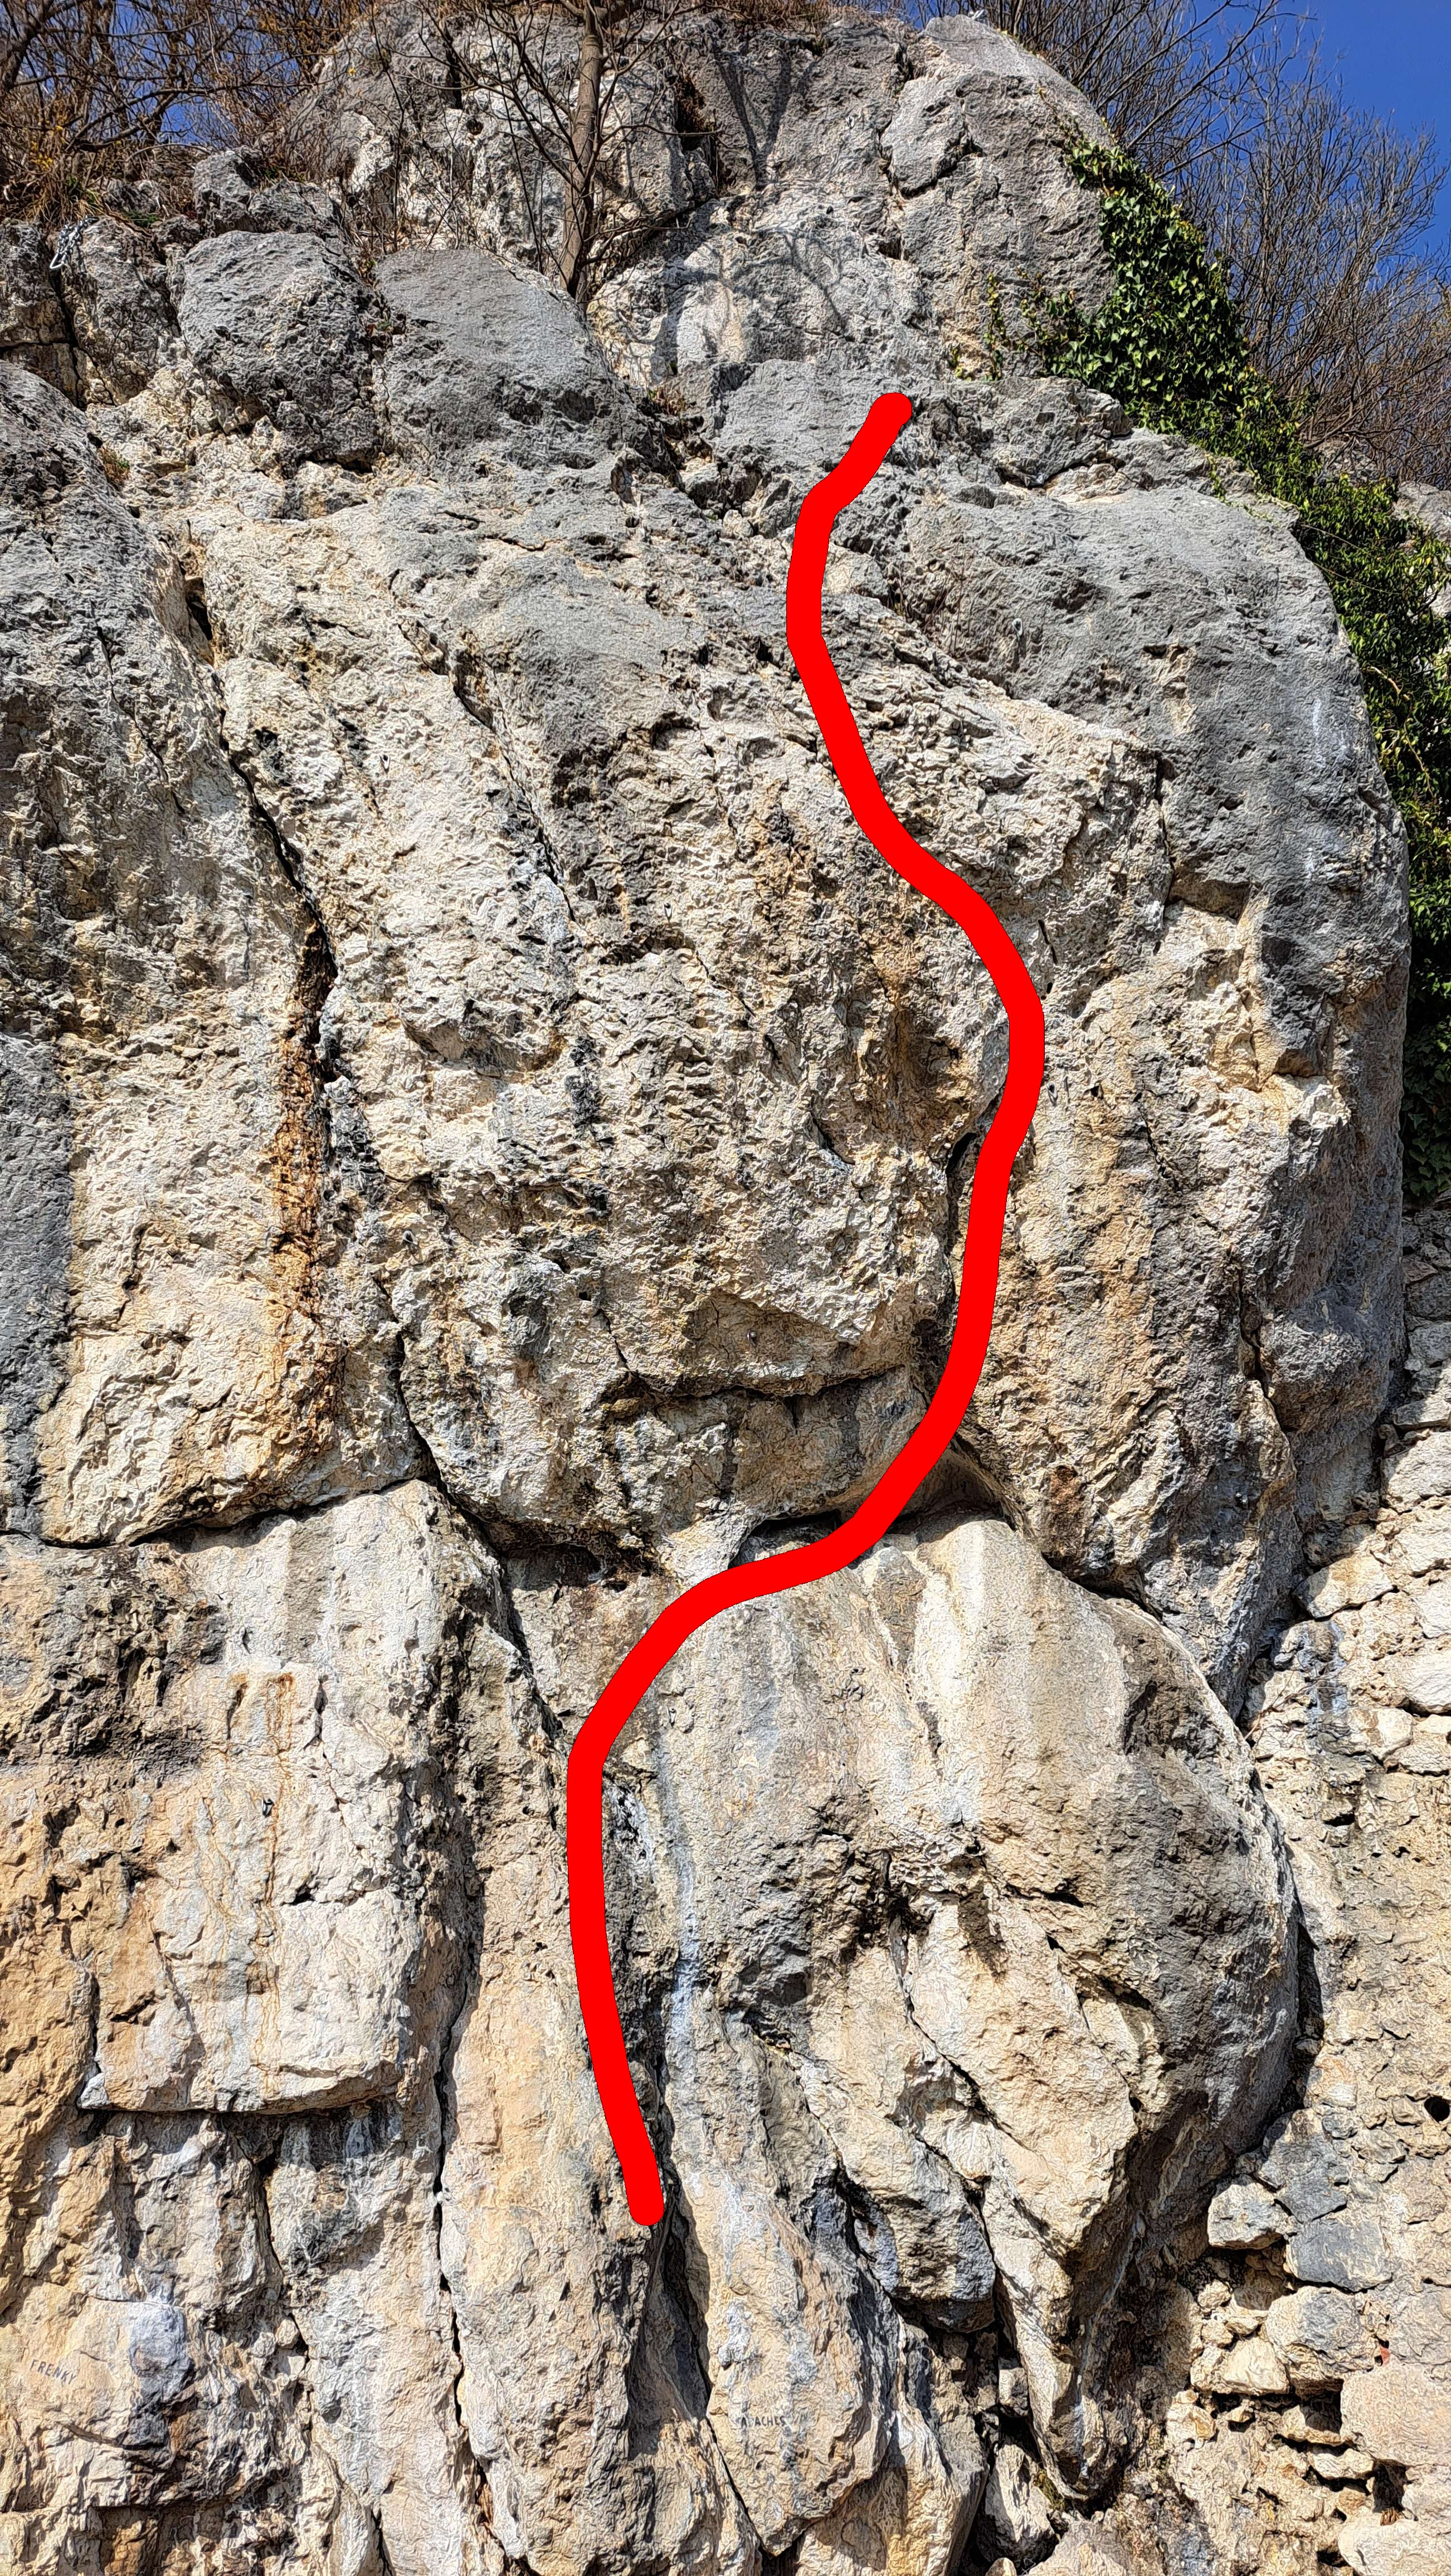
\includegraphics[width=0.4\textwidth]{images/racunalniVid/frame_with_route.jpg}
    \caption{Rezultirajuća slika transformirane linije penjačkog smjera}
    \label{fig:transformacija_perspektive}
\end{figure}

Rezultirajuća slika transformirane linije penjačkog smjera tada se može iscrtati preko slike dobivene sa kamere (slika~\ref{fig:transformacija_perspektive}). Budući da je homografija izračunata na temelju značajki sa stijene, transformirana linija će se precizno poklapati s geometrijom stijene u trenutnom pogledu kamere čime se postiže efekt proširene stvarnosti.